\documentclass{article}
\usepackage[utf8]{inputenc}
\usepackage{graphicx} % Required for inserting images
\usepackage{hyperref}
\usepackage{subcaption}
\usepackage{float}
\usepackage{tcolorbox}
\usepackage{amsmath}
\usepackage{amssymb}
\usepackage{listings}% http://ctan.org/pkg/listings}
\usepackage{algorithm}
\usepackage{algorithmic}
\usepackage[toc,page]{appendix}
%\usepackage[backend=biber]{biblatex}
\usepackage{multicol}
\usepackage{siunitx}
\usepackage{comment}
\usepackage{xcolor}
\usepackage{caption}
\usepackage{forest}
\usepackage{tikz}
\usetikzlibrary{shapes.geometric, arrows}


\tikzstyle{startstop} = [rectangle, rounded corners, 
minimum width=3cm, 
minimum height=1cm,
text centered, 
draw=black, 
fill=red!30]

\tikzstyle{io} = [trapezium, 
trapezium stretches=true, % A later addition
trapezium left angle=70, 
trapezium right angle=110, 
minimum width=3cm, 
minimum height=1cm, text centered, 
draw=black, fill=blue!30]

\tikzstyle{process} = [rectangle, 
minimum width=3cm, 
minimum height=1cm, 
text centered, 
text width=3cm, 
draw=black, 
fill=orange!30]

\tikzstyle{decision} = [diamond, 
minimum width=3cm, 
minimum height=1cm, 
text centered, 
draw=black, 
fill=green!30]
\tikzstyle{arrow} = [thick,->,>=stealth]

% To delete lstlisting caption "Listing x"
%\captionsetup[lstlisting]{labelformat=empty}

\lstdefinestyle{myStyle}{
    belowcaptionskip=1\baselineskip,
    breaklines=true,
    frame=none,
    numbers=none, 
    basicstyle=\footnotesize\ttfamily,
    keywordstyle=\bfseries\color{green!40!black},
    commentstyle=\itshape\color{purple!40!black},
    identifierstyle=\color{black},
    backgroundcolor=\color{white},
}

\lstdefinestyle{cypherStyle}{
    backgroundcolor=\color{white},   % choose the background color
    basicstyle=\footnotesize\ttfamily,        % the size of the fonts that are used for the code
    commentstyle=\itshape\color{purple!40!black},
    keywordstyle=\bfseries\color{green!40!black},
    breakatwhitespace=false,         % sets if automatic breaks should only happen at whitespace
    breaklines=true,                 % sets automatic line breaking
    captionpos=b,                    % sets the caption-position to bottom
    commentstyle=\color{gray},    % comment style
    deletekeywords={},            % if you want to delete keywords from the given language
    escapeinside={\%*}{*)},          % if you want to add LaTeX within your code
    extendedchars=true,              % lets you use non-ASCII characters; for 8-bits encodings only, does not work with UTF-8
    %firstnumber=1000,                % start line enumeration with line 1000
    frame=none,                    % adds a frame around the code
    keepspaces=true,                 % keeps spaces in text, useful for keeping indentation of code (possibly needs columns=flexible)
    language=SQL,                    % the language of the code
    morekeywords={*,IF, REQUIRE, FOR, IS, LOAD, CSV, WITH, HEADERS, MERGE, toFloat, toInteger, date},            % if you want to add more keywords to the set
    numbers=none,                    % where to put the line-numbers; possible values are (none, left, right)
    numbersep=5pt,                   % how far the line-numbers are from the code
    numberstyle=\tiny\color{mygray}, % the style that is used for the line-numbers
    rulecolor=\color{black},         % if not set, the frame-color may be changed on line-breaks within not-black text (e.g. comments (green here))
    showspaces=false,                % show spaces everywhere adding particular underscores; it overrides 'showstringspaces'
    showstringspaces=false,          % underline spaces within strings only
    showtabs=false,                  % show tabs within strings adding particular underscores
    stepnumber=1,                    % the step between two line-numbers. If it's 1, each line will be numbered
    stringstyle=\ttfamily,     % string literal style
    tabsize=2,                       % sets default tabsize to 2 spaces
}

%% Golang definition for listings
%% http://github.io/julienc91/lstlistings-golang
%%
\lstdefinelanguage{Golang}%
  {morekeywords=[1]{package,import,func,type,struct,return,defer,panic,%
     recover,select,var,const,iota,},%
   morekeywords=[2]{string,uint,uint8,uint16,uint32,uint64,int,int8,int16,%
     int32,int64,bool,float32,float64,complex64,complex128,byte,rune,uintptr,%
     error,interface},%
   morekeywords=[3]{map,slice,make,new,nil,len,cap,copy,close,true,false,%
     delete,append,real,imag,complex,chan,},%
   morekeywords=[4]{for,break,continue,range,go,goto,switch,case,fallthrough,if,%
     else,default,},%
   morekeywords=[5]{Println,Printf,Error,Print,},%
   sensitive=true,%
   morecomment=[l]{//},%
   morecomment=[s]{/*}{*/},%
   morestring=[b]',%
   morestring=[b]",%
   morestring=[s]{`}{`},%
}

\lstdefinestyle{golangStyle}{
    captionpos=b,              % sets the caption-position to bottom
    belowcaptionskip=1\baselineskip,
    breaklines=true,
    frame=none,
    numbers=none, 
    basicstyle=\footnotesize\ttfamily,
    keywordstyle=\bfseries\color{green!40!black},
    commentstyle=\itshape\color{purple!40!black},
    identifierstyle=\color{black},
    backgroundcolor=\color{white},
    language=Golang,
}


\title{TFM-FernandoMartín}
\author{Fernando Martín Canfrán}

\begin{document}

\section{Dynamic Pipeline}

\begin{figure}[H]
    \centering
    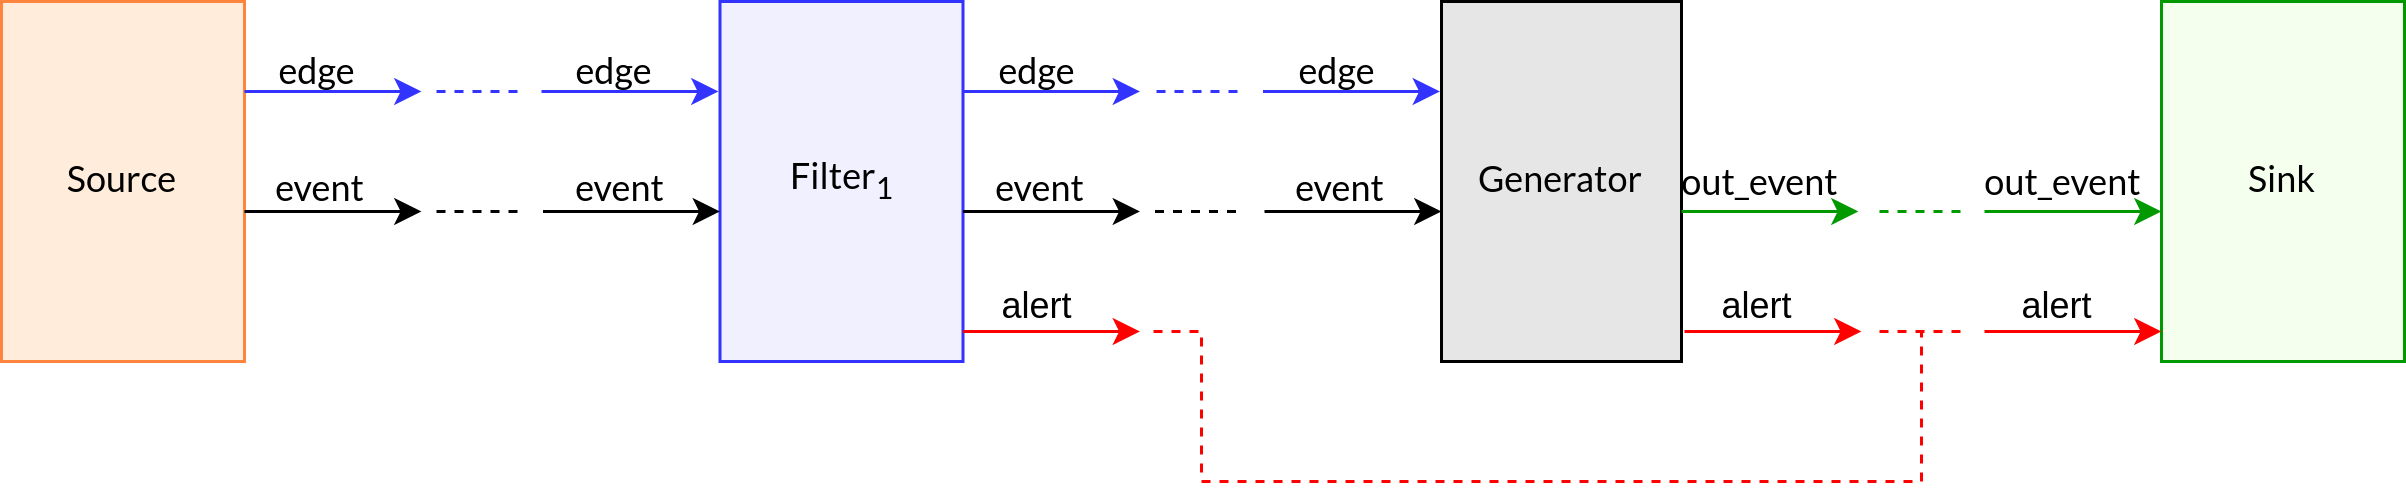
\includegraphics[scale = 0.7]{images/pipeline-schema.png}
    \caption{Pipeline Schema}
    \label{img:pipeline-schema}
\end{figure}

Description of the channels:
\begin{itemize}
    \item \texttt{edge}: only edge dedicated channel
    \item \texttt{event}: events channel
    \item \texttt{alert}: direct channel from the filters (in particular the filter worker) to the sink (it does not go through the Generator, although it has it to be able to give it to the filters so that they are able to write on it)
    \item \texttt{out\_event}: direct dedicated event channel between Generator and Sink.
\end{itemize}

\section{Fraud Patterns}

\subsection{Fraud Pattern I - Card Cloning}

So far, the algorithm (pseudocode) to detect this kind of fraud pattern is the one shown in the algorithm
\ref{alg:check-fraud-1}. Note that $S$ refers to the filter's subgraph and $e_{new}$ is the new incoming edge belonging to the filter, such that it is a opening interaction edge, since in the case it is a closing interaction edge, we do not perform the \text{CheckFraud()}.

\begin{algorithm}[H]
    \small
    \begin{algorithmic}[1]
    \REQUIRE $S$ is the subgraph of edges of the filter (sorted by time)
    \REQUIRE $e_{new}$ is the new incoming opening interaction edge belonging to the filter 
    \STATE $\texttt{fraudIndicator} \gets \texttt{False}$
    \STATE $i \gets |S|$
    \WHILE{$i > 0$ \AND \texttt{fraudIndicator} = \texttt{False}}
      \STATE $e_i \gets S[i]$
      \STATE $\texttt{t\_min} \gets \text{obtain\_t\_min}(e_i, e_{new})$
      \STATE $\texttt{t\_diff} \gets e_{new}.start - e_i.end$
      \IF{$\texttt{t\_diff} < \texttt{t\_min}$}   
        \STATE $\text{createAlert}(e_i, e_{new})$
        \STATE $\texttt{fraudIndicator} \gets \texttt{True}$
      \ENDIF
      \STATE $i \gets i - 1$
    \ENDWHILE
    \end{algorithmic}
    \caption{$\text{CheckFraud}(S, e_{new})$}
    \label{alg:check-fraud-1}
\end{algorithm}

There are some aspects and decisions of this algorithm that are worth to describe:

\begin{itemize}
    \item \textbf{Pairwise detection}. The checking of the anomalous fraud scenario is done doing the check between the new incoming edge $e_{new}$ and each of the edges $e_i$ of the filter's subgraph $S$.
    \item \textbf{Backwards order checking}. The pairs $(e_{new}, e_i)$ are checked in a backwards traversal order of the edge list of the subgraph $S$, starting with the most recent edge of the subgraph and ending with the oldest.  
    \item \textbf{Stop the checking whenever the first anomalous scenario is detected}. Whenever an anomalous scenario corresponding to a pair ($e_{new}, e_i)$, then we stop the checking at this point and emit the corresponding alert. Therefore we do not continue the checking with previous edges of $S$. In what follows we argument the reason why it is sufficient to stop the checking at this point, not having to traverse the full list of edges.
    Assume that we have a subgraph as depicted in Figure x, and that we do not know if there have been anomalous scenarios produced between previous pairs of edges of the subgraph. Name $F_I(X,Y)$ a boolean function that is able to say whether it exists an anomalous fraud scenario of this type between the pair of edges $(X,Y)$ or not. 
    
    We can have that:
    \begin{itemize}
        \item $F_I(B,C)$: ...
        \item $\neg F_I(B,C)$: \dots, 2 possible cases:
        \begin{itemize}
            \item $F_I(A,B)$
            \item $\neg F_I(A,B)$
        \end{itemize}
    \end{itemize}
    \item \textbf{Emission of the pair $(e_{new}, e_i)$ as the alert}. The alert is composed by the pair $(e_{new}, e_i)$ that is detected to cause the anomalous scenario. Both edges are emitted in the alert since we do not know which is the one that is the anomalous. On the one hand, it can be $e_i$, which is previous to $e_{new}$, in the case that $e_i$ at the moment it arrived it did not cause any alert with the previous edges/transactions of the subgraph and it causes it now with a new incoming edge $e_{new}$ which is a regular transaction of the client. On the other hand, it can be $e_{new}$, which is the last having arrived to the system, that it directly causes the alert with the last (ordinary) transaction of the card.
    
    
\end{itemize}

Others -- not so much related with the CheckFraud algorithm, but in general with the filter's algorithm --:
\begin{itemize}
    \item Save all the edges in the subgraph $S$, even though they are the reason of the creation of an anomalous scenario.
\end{itemize}


%\bibliographystyle{plain} % Choose a style (plain, abbrv, unsrt, etc.)
%\bibliography{references} % This points to references.bib  

\end{document}